
The ability to replicate and manipulate voices with high fidelity has far-reaching implications for the fields of cybersecurity and the trustworthiness of information.
To counter possible abuses, one approach involves training binary classifiers, as seen in studies by ~\citep{audiolm,Kharitonov2023SpeakRA,le2023voicebox}. These binary classifiers are trained to detect synthesized audio from authentic real ones.
However, this passive detection approach has significant drawbacks. As generative models advance and the produced content becomes increasingly realistic, the accuracy of these classifiers will progressively decrease. Eventually, distinguishing between authentic and synthesized content could become an extremely difficult, if not impossible, challenge. 
For instance, \citet{le2023voicebox} point out that their classifier mainly recognizes artifacts produced by their model.
For the same reasons, detectors cannot distinguish between different models, diluting the responsibility and accountability of the different actors.
At the same time, regulators and governments (see \citet{ChineseAIGovernance, EuropeanAIAct,  USAIAnnouncement}) are starting to double down on measures to improve transparency and traceability in AI-generated content.

\begin{figure}[b]
    \centering
    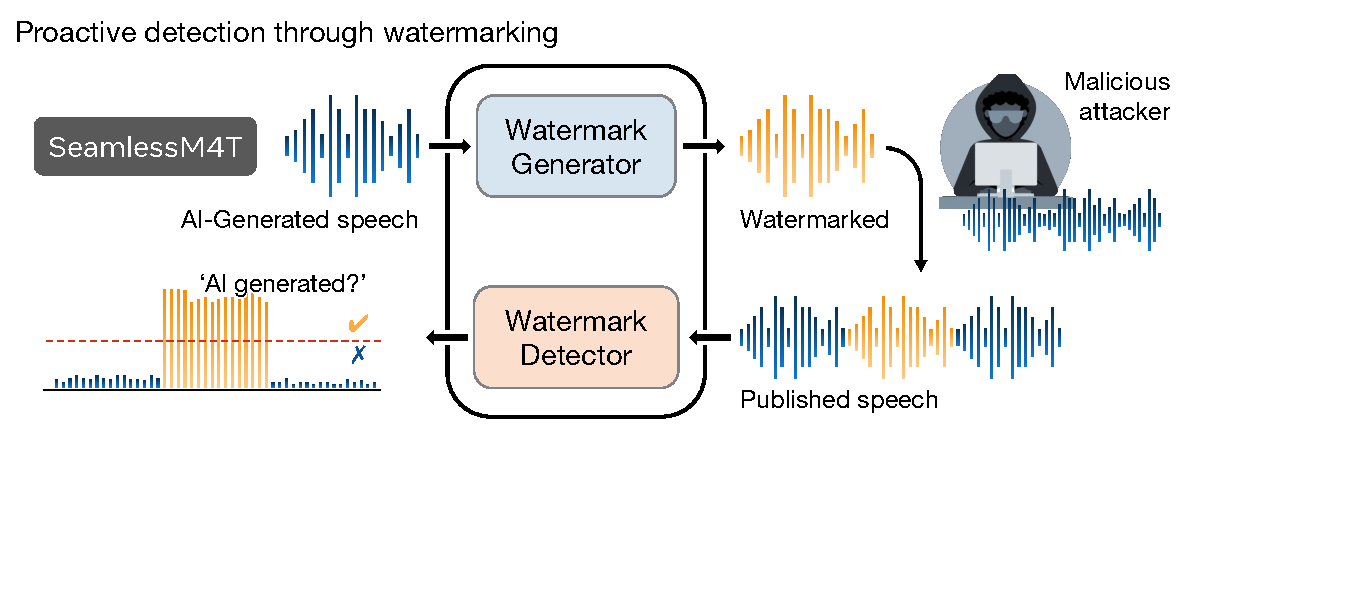
\includegraphics[width=0.75\textwidth, clip, trim={0 1in 1.2in 0.4in}]{figures/rai/wm_fig1.pdf}
    \caption{Proactive detection through watermarking.}
    \label{fig:wm_pipeline}
\end{figure}

We opt for using watermarking as a key strategy for tracing the provenance of AI-generated content~\citep{kirchenbauer2023watermark, fernandez2023stable, wen2023tree, chen2023wavmark}.
Watermarking employs a technique where an undetectable signal is embedded into the audio, which, although imperceptible to human ears, can be easily recognized by specialized algorithms.
This signal can be used to detect if a speech is AI-generated and to identify the specific models used to generate it. 

Most current watermarking methods consider the input audio as a whole indivisible unit when determining if the entire audio is watermarked or not. However, in real-world scenarios, an audio clip often contains a mix of watermarked and non-watermarked parts, in particular in scenarios when synthesized speech is embedded within a larger audio track. This issue is also present in passive detection methods~\citep{le2023voicebox}.
\citet{chen2023wavmark} address this issue by embedding the watermark across one-second intervals within the input audio. For detection, they adopt a brute force approach, sliding through the audio and attempting decoding a watermark starting at each frame. This makes the watermark detection slow and inefficient and constrains the resolution of watermarking to audios larger than one second.
Moreover, current watermarking systems are developed for steganography rather than for detection. They are engineered to hide a binary message (such as 32-128 bits)~\citep{DEAR_Liu0FMZY23,chen2023wavmark} that initially focuses on intellectual property protection rather than tracing provenance or detecting AI-generated content, this overcomplicates the generator and detector architectures.   

In the development of our \seamlesswm model, we have alleviated those limitations by specifically tailoring it for detection purposes drawing conceptual alignments with \citet{juvela2023collaborative}'s approach. Unlike the state-of-the-art methods for audio watermarking \citep{chen2023wavmark} which allows a resolution of generation/detection of only one second, \seamlesswm introduces a significant advancement by enabling the identification of AI-generated audio segments with a precise frame level resolution. 


\begin{figure}[b]
    \centering
    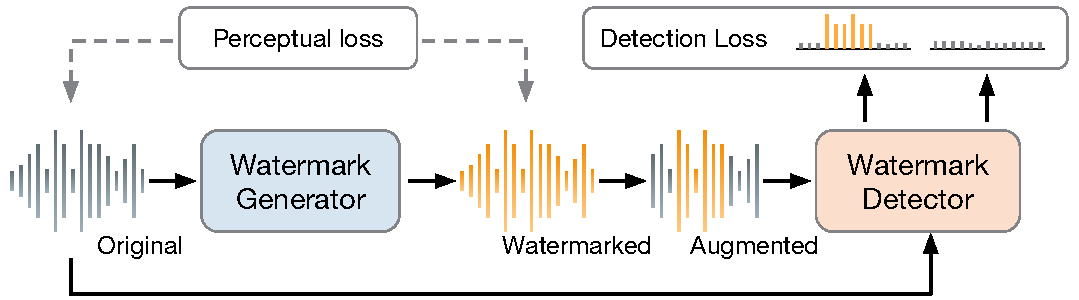
\includegraphics[width=0.6\linewidth, clip, trim={0 -1.5cm 0 0}]{figures/rai/wm_method.pdf}
    \hfill
    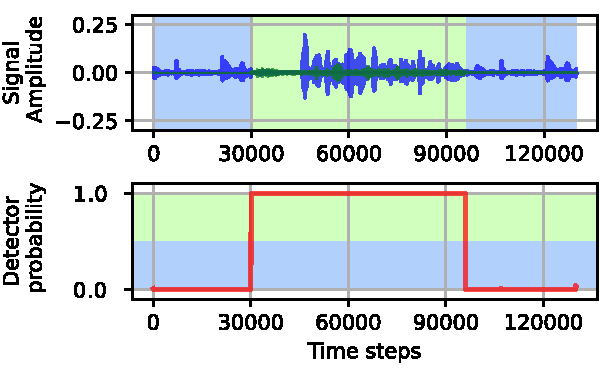
\includegraphics[width=0.36\linewidth, clip, trim={0 0 0 0}]{figures/rai/wm_loca.pdf}
    \vspace{-0.4cm}
    \caption{(Left) Generator-detector training pipeline. (Right) A speech signal, its predicted watermark (green waveform), and detector frame-wise output. A green background color indicates the presence of the watermark.}
    \label{fig:wm_method}
    \label{fig:wm_loc_ex}
\end{figure}


\subsubsection{Methodology}

As illustrated in \Cref{fig:wm_method} we jointly trained a generator and a detector.
The watermarked generator aims to embed a watermark into an audio signal, while the detector aims to detect the watermark at each frame, even in the presence of augmentations.

\paragraph{Training pipeline.} 
We can identify three main steps:
\begin{enumerate}[label=(\roman*), itemsep=4pt, topsep=4pt, leftmargin=20pt]
    \item The watermark generator takes as input a waveform $s \in \mathbb{R}^t$ and outputs a watermark waveform $\delta_w \in \mathbb{R}^t$, where $t$ is the number of frames.
    \item As a first augmentation that happens with probability $0.5$, $k$ windows of the watermark are randomly dropped ($\delta_w$ is set to 0 at these locations).
    They cover approximately 50\% of the total watermark and are built by randomly sampling $k$ starting points and dropping the subsequent $t/2k$ frames.
    The remaining watermark signal is added to the original audio to produce a watermarked audio $s_w = s + \delta_w$.
    Then, a noise layer randomly applies with probability $0.5$ the following augmentations to the watermarked audio: bandpass filter, boost audio, duck audio, echo, highpass filter, lowpass filter, pink noise, gaussian noise, slower, smooth, resample.
    The noise layer helps to improve the watermark's robustness to audio editing, while dropping windows of the watermark greatly helps for localization.
    \item Both the watermarked and original signals are processed through the detector $D$.
    For both of them $D$ outputs a soft decision at every frame, meaning $D(s) \in [0, 1]^t$.
    The detector outputs are illustrated in \Cref{fig:wm_loc_ex}, where we observe that detection happens ($D(s)>0.5$) only when the watermark is present.
\end{enumerate}

\paragraph{Losses.} 
The training minimizes a weighted combination of two losses.
The perceptual loss ensures the watermark is imperceptible. 
It is computed between the original and watermarked audio, as the sum of the Scale Invariant Signal-to-Noise Ratio (SI-SNR) and the L1 loss.
On the other hand, the localization loss ensures robust detection on watermarked audio frames.
When the drop augmentation is applied, it is computed as the binary cross entropy between the detector output (followed by a sigmoid layer) and a binary mask indicating the presence of the watermark.
When it is not applied, the loss is computed over both the original and watermarked audio, and the label is set respectively to 1 and 0.

\begin{figure}[b]
    \centering
    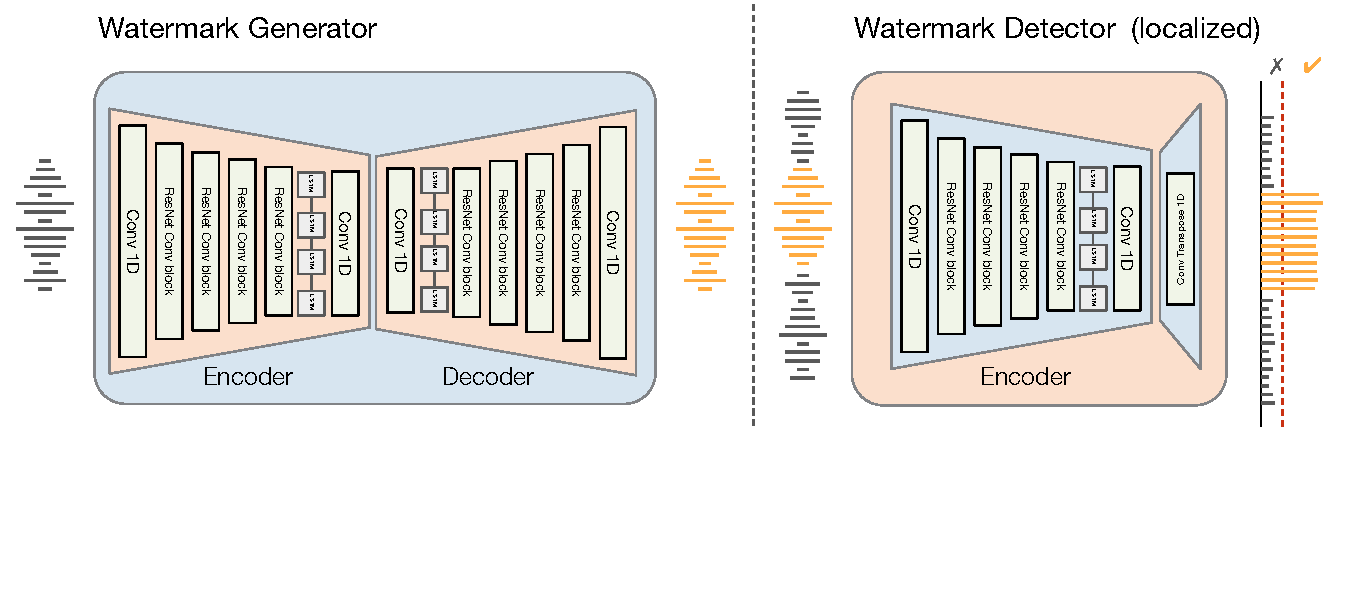
\includegraphics[width=0.99\textwidth, clip, trim={0 1.1in 0in 0in}]{figures/rai/wm_archs.pdf}
    \caption{Architectures of the watermark generator and detector.}
    \label{fig:wm_archs}
\end{figure}

\paragraph{Architectures.} 
The watermark generator (\Cref{fig:wm_archs}) comprises two main components: an encoder and a decoder using main building blocks from~\citep{Defossez2022HighFN}'s.
The encoder model is constructed with a 1D convolution with 32 channels and a kernel size of 7, followed by 4 convolution blocks. 
Each convolution block consists of a singular residual unit succeeded by a down-sampling layer. 
This down-sampling layer employs a strided convolution with a kernel size $K$ equal to twice the stride $S$. 
The residual unit encompasses two convolutions with a kernel size of 3 along with a skip-connection.
Additionally, the number of channels is doubled whenever down-sampling occurs. 
Subsequently, the convolution blocks are succeeded by a two-layer LSTM for sequence modeling and finish in a final 1D convolution layer with a kernel size of 7 and 128 output channels. 
The chosen parameter values for strides $S$ are (2, 4, 5, 8). 
The non-linear activation function is ELU.
The decoder mirrors the encoder but employs transposed convolutions instead of strided convolutions, and the strides in the decoder are applied in the reverse order.

The detector consists of an encoder and a last block made of a transposed convolution and a linear layer.
The encoder shares the same architecture as the one from the generator (but does not share the same weights).
The transposed convolution has eight output channels and upsamples the activation map to the same resolution as the original audio, which results in an activation map with $t \times 8$ channels. 
The linear layer converts the eight dimensions into two, followed by a softmax to have a probability decision at each frame.


\paragraph{Experimental details.}
We trained our models on 4.5k-hour speech data.
This was done on 400k steps, with the Adam optimizer, a learning rate of 3e-4, and a batch size of 32.
We used a sampling rate of 16~kHz and 1s samples, so $t=16000$ in our training.
For the drop augmentation, we used $k=5$ windows of $t/10$ frames.
The weights of the perceptual and localization loss were set to $10$ and $1$.


\subsubsection{Experiments \& Results}
In the following, the results are averaged over 10k samples of 10s from our VoxPopuli validation set unless otherwise specified.

\paragraph{Metrics.} 
To evaluate the quality of the watermarked audio, we used the SI-SNR defined as $\textrm{SI-SNR}(s, s_w) = 10 \log_{10} \left( \| \alpha s \|_2^2 / \| \alpha s - s_w \|_2^2 \right)$, where $\alpha = \langle s, s_w \rangle / \| s \|_2^2$.

To evaluate the quality of the detection, we used True Positive Rate (TPR), i.e., the proportion of watermarked content that is correctly identified, the False Positive Rate (FPR), i.e., the proportion of genuine content incorrectly flagged as watermarked, and accuracy. 

To evaluate the localization task, we used frame accuracy, i.e., the proportion of audio frames correctly labeled, and the Intersection over Union (IoU). 
The latter is defined as the intersection between the predicted and the ground truth detection masks (1 when the frame is watermarked, 0 otherwise), divided by their union: IoU($D(s), gt$)=$|D(s) \cap gt | / |D(s) \cup gt |$. 


\paragraph{Quality and detection results.} 

We first compare detection between active and passive detection using the VoiceBox classifier.
As done in VoiceBox, we masked frames in the spectrogram corresponding to 90\%, 50\%, and 30\% of the phonemes of the utterance before VoiceBox generation. 
We applied \seamlesswm after generation, so the main difference between lines is the distribution of negative samples (AI-generated without watermark).
\Cref{tab:wm_voicebox} highlights that pro-active detection allows for much better detection of synthetic speech than traditional detection, with perfect detection over all the studied samples.

\begin{table}[ht]
    \centering
    \begin{tabular}{r *{3}{c}  *{3}{c}  *{3}{c} }
        \toprule
        & \multicolumn{3}{c}{\textbf{\seamlesswm (Ours)}} & \multicolumn{3}{c}{\textbf{VoiceBox Classif.}} \\
        \cmidrule(rr){2-4} \cmidrule(rr){5-7}
        \textbf{\% Mask} & Accuracy & Precision & Recall & Accuracy & Precision & Recall \\
        \midrule
         \multicolumn{7}{l}{\emph{Original audio vs AI-generated audio}} \\
        30\% & 1.0 & 1.0 & 1.0 & 1.0 & 1.0 & 1.0 \\
        50\% & 1.0 & 1.0 & 1.0 & 1.0 & 1.0 & 1.0 \\
        90\% & 1.0 & 1.0 & 1.0 & 1.0 & 1.0 & 1.0 \\
        \midrule
        \multicolumn{7}{l}{\emph{Re-synthesized audio vs AI-generated audio}} \\
        30\% & \textbf{1.0} & \textbf{1.0} & \textbf{1.0} & 0.704 & 0.714 & 0.680 \\
        50\% & \textbf{1.0} & \textbf{1.0} & \textbf{1.0} & 0.809 & 0.796 & 0.831 \\
        90\% & \textbf{1.0} & \textbf{1.0} & \textbf{1.0} & 0.907 & 0.881 & 0.942 \\
        \hline
    \end{tabular}
    \caption{Comparison with VoiceBox binary classifier. 
    }
    \label{tab:wm_voicebox}
\end{table}


We further compared \seamlesswm to the concurrent deep watermarking method \wavmark.
\Cref{tab:wm_robustness} shows the detection results for different augmentations applied before detection.
Compared to \wavmark, we obtained better or similar detection results, with consistently better audio quality.
The average SI-SNR between the original and watermarked audio is 37.82~dB, while \wavmark achieves 33.7~dB.


\begin{table}[ht]
    \centering
    \begin{tabular}{l l *{3}{l}  *{3}{l}}
        \toprule
        & & \multicolumn{3}{c}{\textbf{\seamlesswm (Ours)}} & \multicolumn{3}{c}{\textbf{\wavmark}} \\
        \cmidrule(rr){3-5} \cmidrule(rr){6-8}
        & SI-SNR & \multicolumn{3}{c}{\textbf{37.82}} & \multicolumn{3}{c}{33.69} \\
        \midrule
        \midrule
        && TPR & FPR & Acc & TPR & FPR & Acc \\
        \cmidrule(rr){3-5} \cmidrule(rr){6-8} 
        &No Attack   & 1.00  & 0.00 & \textbf{1.00}
                        & 0.99 & 0.00 & 0.99 \\
        \cmidrule(rr){2-8}
        \multirow{11}{*}{\rotatebox[origin=c]{90}{Robustness Attacks}} 
        &Bandpass Filter & 1.00 & 0.00 & \textbf{1.00}   
                        & 0.99 & 0.00 & 0.99 \\
        &Highpass Filter & 1.00 & 0.00 & \textbf{1.00} 
                        & 0.99 & 0.00 & 0.99 \\
        &Lowpass Filter & 1.00 & 0.00 & \textbf{1.00} 
                        & 0.99 & 0.00 & 0.99 \\
        &Boost Audio & 1.00 & 0.00 & \textbf{1.00}
                        & 0.99 & 0.00 & 0.99 \\
        &Duck Audio & 1.00 & 0.00 & \textbf{1.00}
                        & 0.99 & 0.00 & 0.99 \\
        &Echo & 1.00 & 0.00 & \textbf{1.00}
                        & 0.85 & 0.00 & 0.92 \\
        &Pink Noise & 1.00 & 0.00 & \textbf{1.00}
                        & 0.99 & 0.00 & 0.99 \\
        &Random Noise & 1.00 & 0.00 & \textbf{1.00}
                    & 0.91 & 0.00 & 0.95 \\
        &Slower & 1.00 & 0.00 & \textbf{1.00} 
                    & 0.00 & 0.00 & 0.50 \\
        &Smooth & 1.00 & 0.00 & \textbf{1.00}
                & 0.96 & 0.00 & 0.98 \\
        &Updown Resample & 1.00 & 0.00 & \textbf{1.00}
                        & 0.99 & 0.00 & 0.99 \\
        \hline
    \end{tabular}
    \caption{Metrics (TPR/FPR/accuracy) for different edits applied before detection. FPR is computed empirically on 10k samples.}
    \label{tab:wm_robustness}
\end{table}


\paragraph{Localization results.} 
To have frame-wise localization with \wavmark, we used their brute-force-detection: a window of 1s slides over the 10s of speech with the default shift value of 0.05s. 
The first 16 decoded bits (over 32) were used to detect if the window is watermarked.
Whenever a watermarked window is detected, we labeled the 16k frames of the window as watermarked, and we ended up with a detection mask in $\{0,1\}^t$.

We plot in \Cref{fig:wm_localization_quant} the mean frame accuracy and IoU of \seamlesswm and \wavmark for different proportions of watermarked speech into the non-watermarked speech.
Our approach achieves an impressive IoU of 0.99 when just one second of speech is AI-manipulated, compared to \wavmark's 0.35.
\seamlesswm allows for precise detection of minor audio alterations: it can pinpoint AI-generated segments in audio down to the frame level (1/16k secs), while the concurrent \wavmark only provides one-second resolution and therefore lags behind in terms of IoU. 
This is especially relevant for speech samples, where a simple word modification may greatly change meaning. 

\begin{figure}
    \centering
    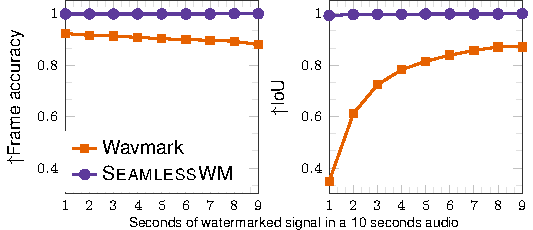
\includegraphics[width=.7\textwidth]{figures/rai/watermarking_accuracy_miou.pdf}
    \caption{Localization results for frame-wise watermark detection.}
    \label{fig:wm_localization_quant}
\end{figure}

